\documentclass[9pt]{beamer}

\usetheme[{titleformat plain}=smallcaps,
           titleformat title=smallcaps,
           titleformat subtitle=regular,
           titleformat section=smallcaps,
           titleformat frame=smallcaps,
           numbering=fraction,
          ]{metropolis}
\usepackage{appendixnumberbeamer}
\geometry{paperwidth=213.3mm,paperheight=120mm}

\usepackage{../_style/common}
\usepackage{../_style/defs}
\usepackage{emoji}

\graphicspath{{pictures/}{../_pictures/}}

\title{Data and Interfaces}
\subtitle{
    \itshape
    successful abstractions as building blocks
}
\date{October, 2022}
\author{Alessandro Candido}
\titlegraphic{
    \vfill\vspace*{250pt}
    
\includegraphics[height=1cm]{../_logos/unimi_logo.png}\hfill
    
\includegraphics[height=1cm]{../_logos/infn_logo.png}\\
}

\begin{document}

\maketitle

\setlist[description]{font=\quad\normalfont\bfseries\scshape\space}
\metroset{block=fill}


\begin{frame}{Who am I?}
    \begin{columns}
        \begin{column}{0.5\textwidth}
            I am a \textbf{PhD student} in \textbf{HEP theory}, about to
            finish.\newline

            Since my Master I have spent a significant part of my research
            working on \alert{\textbf{software projects}}, with an increasing
            number of collaborators.\newline

            \vspace*{5pt}
            \partitle{References}
            \vspace*{5pt}

            Now, as part of \nnpdf{}, I had to work and organize projects with
            $\order{5\text{-}10}$ developers -- not incredibly many, but already
            \textit{\textbf{challenging}}.\newline

            Moreover, personal projects driven me to explore beyond the
            boundaries of what is useful for physics.
            With less \sout{pressure} needs you can explore more\dots but often
            not as deep.\newline

            \vspace*{5pt}
            \partitle{My Goal}
            \vspace*{5pt}

            I am not here to teach, but just to \textbf{share my experience}.
            This is compliant with the references.
        \end{column}
        \begin{column}{0.5\textwidth}
            \begin{figure}
                \centering
                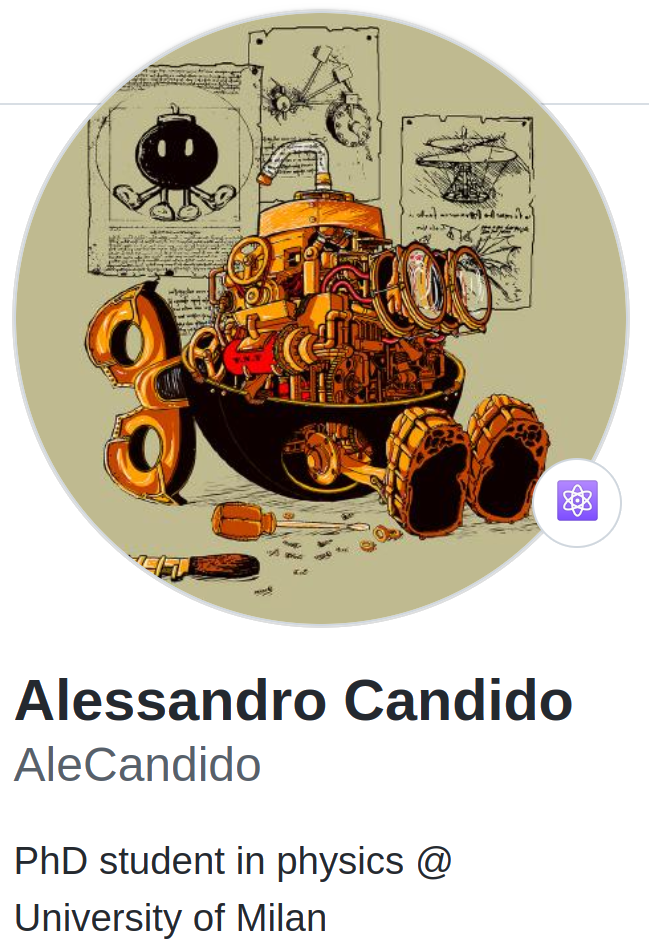
\includegraphics[width=0.5\textwidth]{mygh}
            \end{figure}
        \end{column}
    \end{columns}
\end{frame}

% \begin{frame}{The Role of Trade-offs}
    % \begin{columns}
        % \begin{column}{0.5\textwidth}
            % \vspace*{20pt}
            % \begin{center}
                % \itshape\bfseries 
                % There are no absolute truths.
            % \end{center}
            % \begin{flushright}
                % \itshape
                % -- is this an absolute truth? \emoji{thinking-face}
            % \end{flushright}

            % \vspace*{10pt}
            % In a sense, problems might look similar, even when they are not
            % that much\dots
            % \vspace*{20pt}
            
            % \begin{figure}
                % \centering
                % 
\includegraphics[width=\textwidth]{solution}
                % \caption{
                    % Artistic view of the solution function, over the space of
                    % problems.
                % }
            % \end{figure}
        % \end{column}
        % \begin{column}{0.5\textwidth}
            % So, better to know many possible solutions, and always consider
            % multiple alternatives.

            % \vspace*{10pt}
            % \begin{figure}
                % \centering
                % 
\includegraphics[width=0.6\textwidth]{balancing}
            % \end{figure}
            % \vspace*{10pt}

            % Moreover
            % \href{https://en.wikipedia.org/wiki/All_that_glitters_is_not_gold\#In_popular_culture}{\enquote{All
            % that is gold does not glitter}}, not all good solutions are
            % manifest.
        % \end{column}
    % \end{columns}
% \end{frame}

\begin{frame}{Outline}
    \vspace*{10pt}
    \begin{center}
        \itshape
        The task I have been given is to discuss \textbf{interfaces} and
        \textbf{data management.}
    \end{center}
    \vspace*{10pt}

    \begin{columns}
        \begin{column}{0.5\textwidth}
            \alert{\textbf{Python}} is not the \enquote{best} programming
            language, nor the unique one.
            But Python is definitely a successful one.
            \vspace*{10pt}

            And the success for a language is mostly determined by the
            availability of \textbf{libraries} and
            \textbf{applications}\footnote{
                There are relevant and determinant language features, and for
                Python is its \textbf{expressiveness}, that is fundamental for
                new users and \textit{\textbf{maintainability}}.
            }.\newline

            In the case of Python:
            \begin{description}
                \item[application] scientific computation, and data science\footnote{
                    Part of the success has been due to \textit{web
                    frameworks}, but it is less relevant nowadays.
                }
                \item[libraries] Numpy, Scipy, Pandas, Xarray, \dots
            \end{description}
            \vspace*{30pt}

            Of course ML frameworks now play a big a role, but it is almost a
            consequence\dots
            \vspace*{5pt}
        \end{column}
        \begin{column}{0.5\textwidth}
            So, in a sense, the advantage of Python is that its
            \alert{\textbf{libraries}} can be \alert{\textbf{written not in
            Python}}.

            But in order this to be possible, it is crucial to build a
            successful \textbf{abstraction}.
            \vspace*{20pt}

            \begin{enumerate}
                \item abstractions
                \item interfaces
                \item examples
                \item project management
            \end{enumerate}
            \vspace*{20pt}

            \begin{figure}
                \centering
                
\includegraphics[height=0.15\textwidth]{python}
                \hspace*{20pt}
                
\includegraphics[height=0.15\textwidth]{numpy}
                \hspace*{20pt}
                
\includegraphics[height=0.15\textwidth]{pandas}
                \hspace*{20pt}
                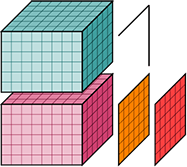
\includegraphics[height=0.15\textwidth]{xarray}
            \end{figure}
            \vspace*{10pt}
        \end{column}
    \end{columns}
\end{frame}

\section{Abstractions}

\begin{frame}{Concepts}
    \begin{center}
        \textbf{Abstractions} are useful because they \textbf{encode concepts}.
    \end{center}
    \vspace*{30pt}

    \begin{columns}
        \begin{column}{0.1\textwidth}
        \end{column}
        \begin{column}{0.4\textwidth}
            \vcinclude{numpy}{height=50pt} {\Huge $\,\quad\to\qquad$} N-dim array
            \vspace*{10pt}

            \vcinclude{pandas}{height=50pt} {\Huge $\qquad\to\qquad$} Table
        \end{column}
        \begin{column}{0.4\textwidth}
            \vcinclude{xarray}{height=50pt} {\Huge $\.\quad\to\qquad$} Dataset
            \vspace*{10pt}

            \vcinclude{networkx}{height=50pt} {\Huge $\qquad\to\qquad$} Network
        \end{column}
        \begin{column}{0.1\textwidth}
        \end{column}
    \end{columns}
    \vspace*{10pt}
    \begin{flushright}
        \footnotesize
        Many useful libraries implement tools to \textbf{perform an action},
        not only to manage data structures.
    \end{flushright}
    \vspace*{10pt}

    It is crucial to \textit{hide} implementation \textit{details}
    ($\sim$ \textbf{encapsulation}).

    Often fundamental for the solution, and understanding them can improve the
    usage.\newline
    But they add a huge cost for the user: hard to learn, depend on the
    internals.

    \begin{flushright}
        \footnotesize
        Check more among NumFOCUS
        \href{https://numfocus.org/sponsored-projects}{sponsored} and
        \href{https://numfocus.org/sponsored-projects/affiliated-projects}{affiliated}
        projects.
    \end{flushright}
\end{frame}

\begin{frame}{Building Blocks}
    \begin{columns}
        \begin{column}{0.5\textwidth}
            On one side Python is a terrible language to build abstractions:
            everything is \textbf{exposed}.
            \begin{figure}
                \centering
                
\includegraphics[width=0.2\textwidth]{capsule}
            \end{figure}

            On the other, it is a perfect one: it relies on \textbf{duck typing}.
            \begin{figure}
                \centering
                
\includegraphics[width=0.3\textwidth]{duck.png}
            \end{figure}

            \begin{center}
                \itshape
                If it looks like a duck, swims like a duck, and quacks like a
                duck, then it is a duck.
            \end{center}
        \end{column}
        \begin{column}{0.5\textwidth}
            Each well-behaving object can be used as an \textbf{effective
            building block} inside a more complex infrastructure.
            \vspace*{20pt}

            \begin{figure}
                \centering
                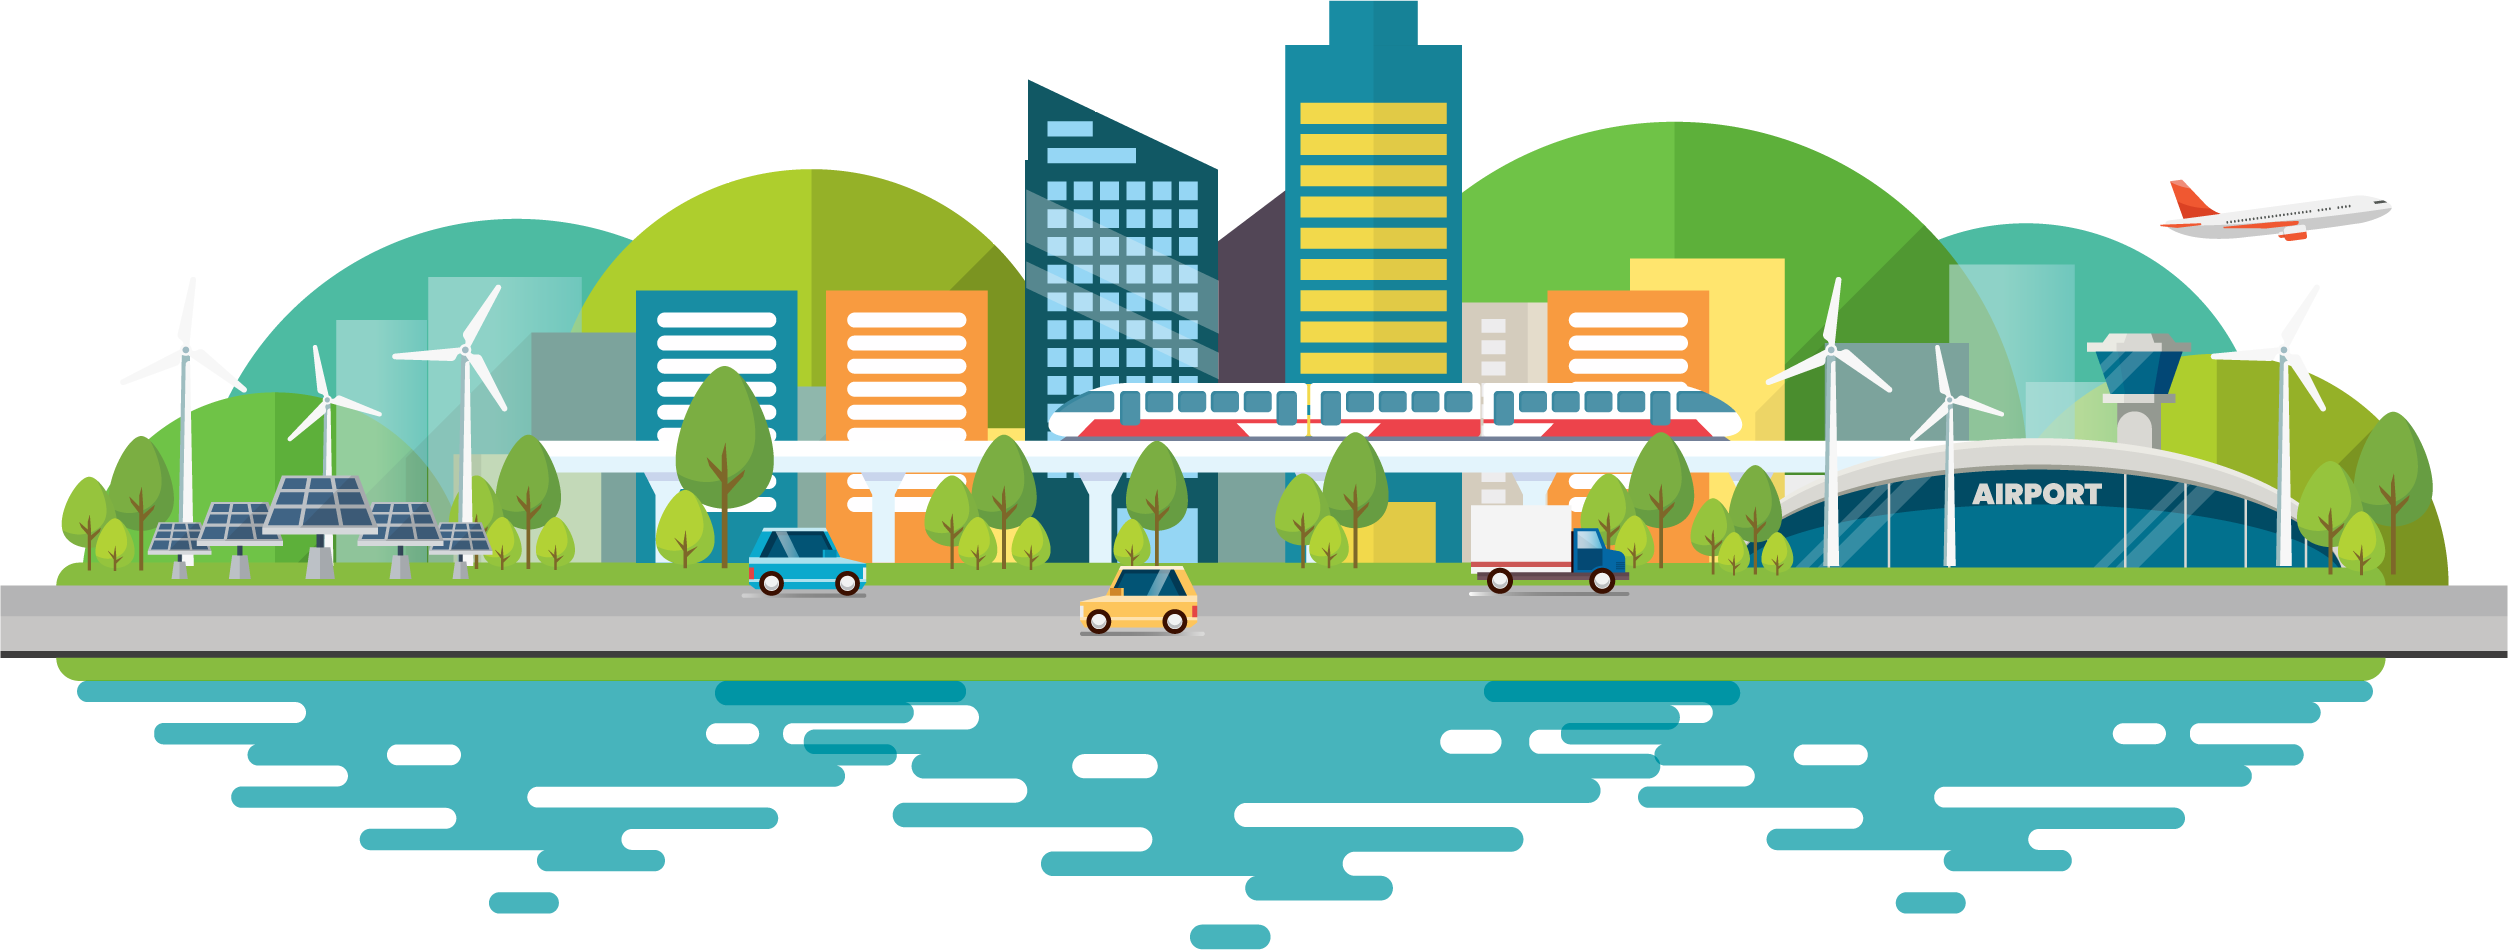
\includegraphics[width=0.8\textwidth]{infrastructure}
            \end{figure}
            \vspace*{20pt}

            The essential concept to tame complexity is modularity\footnote{
                Objects are definitely useful, but not mandatory.
            }.
        \end{column}
    \end{columns}
\end{frame}

\section{Interfaces}

\begin{frame}[fragile]{What is an interface?}
    \vspace*{30pt}
    \begin{columns}
        \begin{column}{0.02\textwidth}
        \end{column}
        \begin{column}{0.47\textwidth}
            Some programming languages define an explicit concept of interface:

            \begin{lstlisting}[language=Go,style=mystyle]
// Go example, see full at: https://gobyexample.com/interfaces
type geometry interface {
    area() float64
    perim() float64
}

type rect struct {
    width, height float64
}
// Implement geometry on rects.
func (r rect) area() float64 {
    return r.width * r.height
}
// [...]

// Call methods that are in the named interface.
func measure(g geometry) {
    fmt.Println(g)
    fmt.Println(g.area())
    fmt.Println(g.perim())
}\end{lstlisting}

            In its most basic instance, it is just an object that expose a
            property (also a specific attribute in Plain Old Data, POD).
        \end{column}
        \begin{column}{0.47\textwidth}
            This is intrinsic in OOP, e.g.\ C++\footnote{
                where no explicit interface feature is present
            } gets extremely close through pointers and
            \href{https://en.wikipedia.org/wiki/Polymorphism_(computer_science)}{polymorphism}.

            \begin{lstlisting}[language=C++,style=mystyle]
// C++ example, see full at: https://cplusplus.com/doc/tutorial/polymorphism/
class Polygon {
  protected:
    int width, height;
  public:
    void set_values (int a, int b)
      { width=a; height=b; }
};

class Rectangle: public Polygon {
  public:
    int area()
      { return width*height; }
};

int main () {
  Rectangle rect;
  Polygon * ppoly1 = &rect;
  ppoly1->set_values (4,5);
  cout << rect.area() << '\n';
  return 0;
}\end{lstlisting}
        \end{column}
        \begin{column}{0.02\textwidth}
        \end{column}
    \end{columns}
\end{frame}

\begin{frame}[fragile]{More Abstract}
    \vspace*{30pt}
    \begin{columns}
        \begin{column}{0.5\textwidth}
            Interfaces exists also \textbf{independently from} any specific
            \textbf{language} feature.

            \begin{center}
                \itshape
                They are \alert{contracts} between two or multiple parties, on
                a certain behavior.
            \end{center}

            Consider that the word \enquote{interface} is also in \textit{API
            (application programming interface)} and \textit{ABI (application
            binary interface)}.\newline

            \begin{figure}
                \centering
                
\includegraphics[width=0.5\textwidth]{contract}
            \end{figure}

            E.g. an API is a contract between developers/source codes, while an
            ABI is an agreement at the level of the compiled code.
        \end{column}
        \begin{column}{0.5\textwidth}
            Another example of interface is a \textbf{Foreign Function
            Interface (FFI)}, that is a way to call code from a different
            language (\alert{fundamental in Python}, more later).
            \vspace*{10pt}

            \begin{lstlisting}[language=Python,style=mystyle]
import ctypes
libc = ctypes.CDLL('/lib/libc.so.6')  # Under Linux/Unix
t = libc.time(None)  # Equivalent C code: t = time(NULL)
print(t)\end{lstlisting}
            \vspace*{20pt}

            Interfaces are a concept (or a
            \href{https://refactoring.guru/design-patterns}{design pattern})
            you can also use to build other concepts upon.\newline

            E.g.\ a \href{https://en.wikipedia.org/wiki/Mixin}{mixin}, leverage
            a specific behavior (an interface), to provide some other features
            to your object\footnote{
                Specifically related to OOP and inheritance.
            }.
        \end{column}
    \end{columns}
\end{frame}

\begin{frame}{Template}
    \begin{columns}
        \begin{column}{0.5\textwidth}
            Another option to interface two different programs is to have them
            talking through files.\newline

            An agreement over a \textbf{file structure} is an interface.
            \begin{flushright}
                \footnotesize
                File structure is more than just the language (e.g.\ a
                \texttt{YAML} file).

                \hspace*{10em} The language specify just the
                \textbf{\textit{syntax}}, while a proper interface should
                specify also the \textbf{\textit{semantics}}.
            \end{flushright}

            \begin{figure}
                \centering
                
\includegraphics[width=0.2\textwidth]{data-file}
            \end{figure}

            In general, you can implement the concept \alert{\textbf{in data}},
            e.g.\ including memory exchange of \textit{text} or \textit{binary
            blobs} (think about in memory databases).

            \begin{flushright}
                \footnotesize
                In practice, apart from specific needs, it is convenient to use
                files.
            \end{flushright}
        \end{column}
        \begin{column}{0.5\textwidth}
            Actual encapsulation.
            (Use methods, properties, and functions, not directly attributes.
            Only when required, otherwise attributes are good enough.)

            Methods are useful, not required. Make clever use of functions that
            act on specific objects.
            (Also because Python does not allow for many \texttt{impl} blocks,
            so required to split over multiple files).
        \end{column}
    \end{columns}
\end{frame}

\begin{frame}{In Python}
    \begin{columns}
        \begin{column}{0.5\textwidth}
            Plain Old Data POD.
            (Best implemented with dataclasses, see after.)

            Actual encapsulation.
            (Use methods, properties, and functions, not directly attributes.
            Only when required, otherwise attributes are good enough.)

            Practical use of duck typing.

            Use modules and classes as namespaces.
            (Consider expose better public API, hiding internals, e.g.
            \texttt{\_internal}).
        \end{column}
        \begin{column}{0.5\textwidth}
            The static analyzer is your best friend (the best replacement for
            the compiler).

            Writing explicit code helps the analyses.

            When possible, give hints with types (but do not break duck typing
            when not required).

            Also, in Python itself you can find the concept of interface
            (protocol, e.g.\ a
            \href{https://docs.python.org/3/glossary.html\#term-sequence}{sequence})
            implemented at many levels:

            \begin{description}
                \item[C API] at the level of C implementation\footnote{
                        \texttt{CPython} specific
                    }, the
                    \href{https://docs.python.org/3/c-api/sequence.html}{Sequence
                    Protocol}
                \item[typing] in the type hinting system,
                    \href{https://docs.python.org/3/library/typing.html?highlight=sequence\#typing.Sequence}{\texttt{typing.Sequence}}
                \item[runtime] consumable in code itself,
                    \href{https://docs.python.org/3/library/collections.abc.html?highlight=sequence\#collections.abc.Sequence}{\texttt{collections.abc.Sequence}} 

            \end{description}
        \end{column}
    \end{columns}
\end{frame}

\section{Examples}

\begin{frame}{Template}
    \begin{columns}
        \begin{column}{0.5\textwidth}
            When possible: No dicts, no strings.

            Attributes

            Properties

            Dataclasses
            (Because Python has no POD, best way to enforce a certain
            data structure.)

            Enums

            foreign language (Rust, C/C++ if possible, mention Fortran with
            f2py)
        \end{column}
        \begin{column}{0.5\textwidth}
        \end{column}
    \end{columns}
\end{frame}

\section{Project Management}

\begin{frame}{Docs}
    \begin{center}
        Presenting the code is fundamental: since you \textbf{want to have
        users}, it has to be \textit{useful} and \textit{simple}.

        \textit{And everything is \textbf{simple, when} it is
        \alert{\textbf{well explained}}.}
    \end{center}
    \vspace*{10pt}

    \begin{columns}
        \begin{column}{0.35\textwidth}
            It is a synthetic replacement for office hours.
            \vspace*{10pt}

            \begin{itemize}
                \item given a \textbf{question}, the \textbf{answer} should be
                  properly written in the docs; in familiar terms, and simple
                  to find, not only: 
                \item sometimes, it should provide \textbf{answers before
                  questions} (since it is not always clear which are the proper
                  ones)
            \end{itemize}

            \begin{figure}
                \centering
                
\includegraphics[width=0.6\textwidth]{question-docs}
            \end{figure}
        \end{column}
        \begin{column}{0.35\textwidth}
            Good documentation have to provide resources for different users,
            so they need to be \textbf{hierarchical}.
            \vspace*{10pt}

            \begin{description}
                \item[presentation] a \textbf{home page}, to meet new users,
                    and a starting point
                \item[getting started] \textbf{tutorials}, to begin hands on
                \item[user manual] to answer most of the common needs
                \item[reference] a complete explanation of the public interface
            \end{description}
        \end{column}

        \begin{column}{0.3\textwidth}
            \begin{figure}
                \centering
                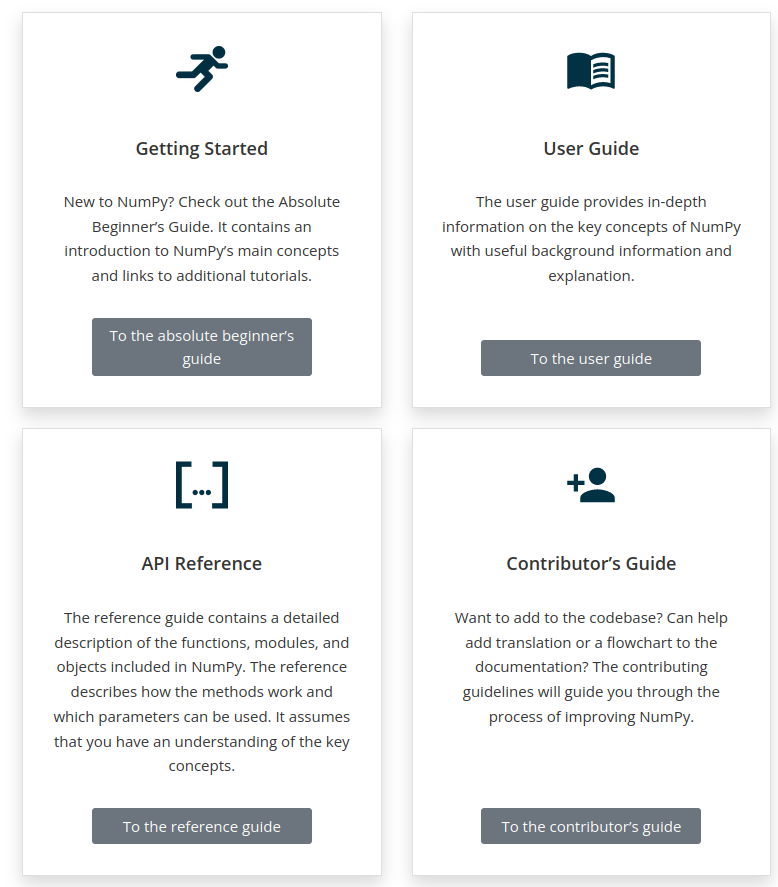
\includegraphics[width=\textwidth]{numpy-hierarchical-docs}
                \caption{
                    Numpy docs \href{https://numpy.org/doc/stable/}{starting page}.
                }
            \end{figure}

            % In general, it is convenient to document everything (e.g.\ with
            % docstrings), but the internals are for developers and
            % maintainability, not for users\footnote{
                % There should be a clear distinction, but they are both
                % important.
            % }.
            % \vspace*{10pt}
        \end{column}
    \end{columns}
\end{frame}

\begin{frame}{Home and Tutorials}
    \begin{columns}
        \begin{column}{0.5\textwidth}
            \vspace*{5pt}

            A good landing page is fundamental:
            \begin{itemize}
                \item a \textbf{unique reference} point
                \item communicate the \textbf{target audience}, and
                \item the scope and \textbf{goal} of the project
            \end{itemize}

            \begin{figure}
                \centering
                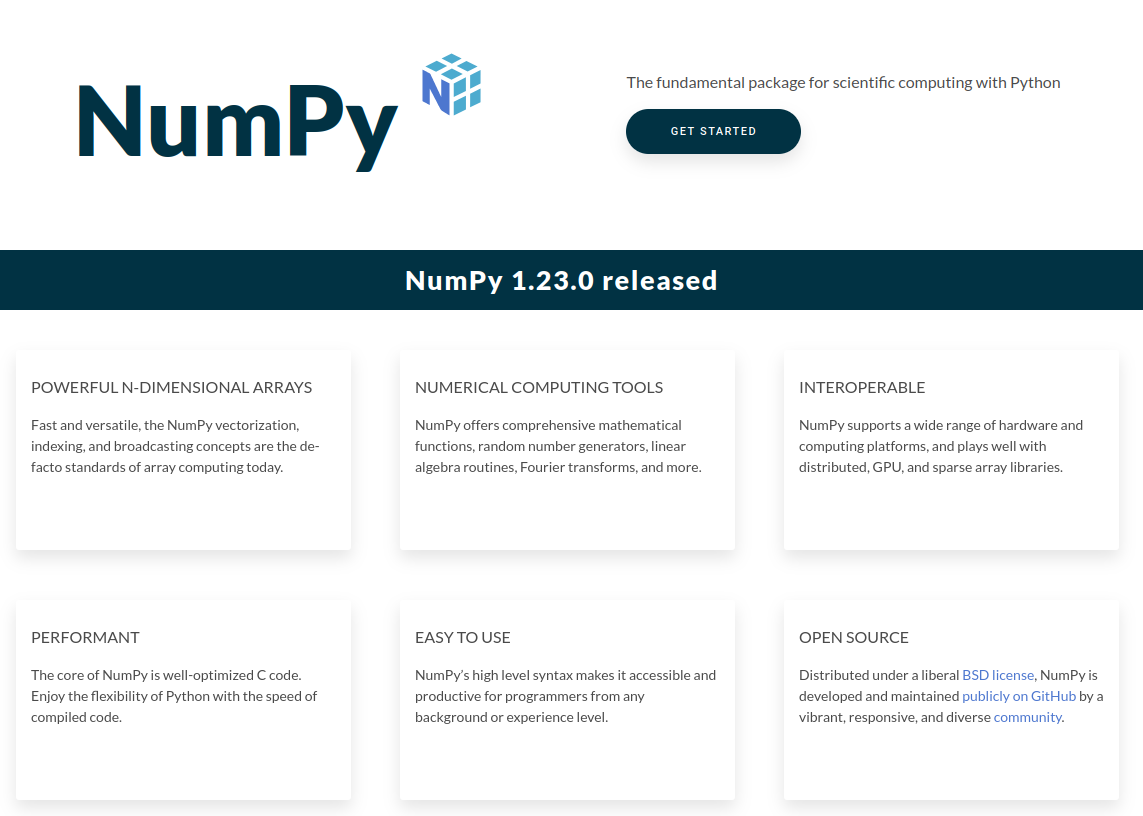
\includegraphics[width=0.8\textwidth]{numpy-home}
                \caption{Numpy \href{https://numpy.org/}{home}.}
            \end{figure}
            
            All the \textbf{relevant pointers} should be here, but only top
            level (think of a \textit{logarithmic navigation}).
        \end{column}
        \begin{column}{0.5\textwidth}
            \vspace*{10pt}

            \textbf{Tutorials} should be a \textit{\textbf{walk-through}}, the
            user has to know nothing but the initial problem.
            \vspace*{5pt}

            Jupyter notebooks are very useful, with explanations and outputs.
            \vspace*{5pt}

            \begin{figure}
                \centering
                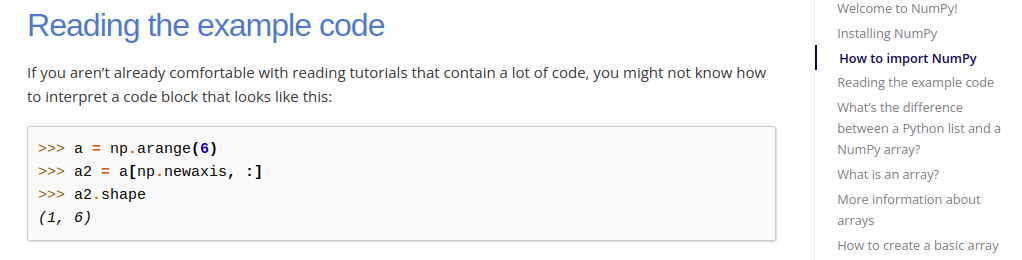
\includegraphics[width=0.9\textwidth]{numpy-abs-beginners}
                \caption{
                    Numpy
                    \href{https://numpy.org/doc/stable/user/absolute_beginners.html}{absolute
                    beginners} guide.
                }
            \end{figure}

            Consider to incrementally collect good examples. If easily
            discoverable they can be extremely useful.
            \vspace*{5pt}

            \begin{figure}
                \centering
                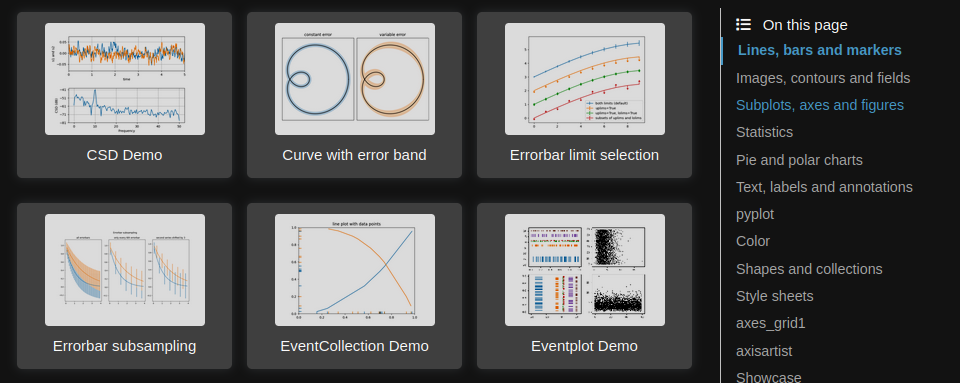
\includegraphics[width=0.8\textwidth]{matplotlib-gallery}
                \caption{
                    Matplotlib
                    \href{https://matplotlib.org/stable/gallery/}{gallery}
                }
            \end{figure}
        \end{column}
    \end{columns}
\end{frame}

\begin{frame}{Dependencies}
    \begin{columns}
        \begin{column}{0.5\textwidth}
            Another crucial point is \textbf{dependencies picking}.
            \vspace*{10pt}

            Trade-off:
            \begin{description}
                \item[pro] software reuse: deduplication, leverage other people work
                \item[con] sync versions, rely on external maintenance
            \end{description}
            \vspace*{20pt}

            So, what if one wants the \textbf{\textsc{pros}} and not the
            \textbf{\textsc{cons}}?

            Mitigate the issues with \textit{optimal choices}:
            \begin{itemize}
                \item \alert{\textbf{community}} or company projects (not
                  single maintainer)
                \item \alert{\textbf{stable}} enough (not early stage)
                \item still \alert{\textbf{active}} (not abandoned)
            \end{itemize}
            \vspace*{10pt}

            The other option is to pick a project, though unstable or inactive,
            and accept to maintain it yourself, in case you need.
        \end{column}
        \begin{column}{0.5\textwidth}
            \begin{figure}
                \centering
                \begin{tcolorbox}[size=tight,sharpish corners,boxrule=0mm]
                    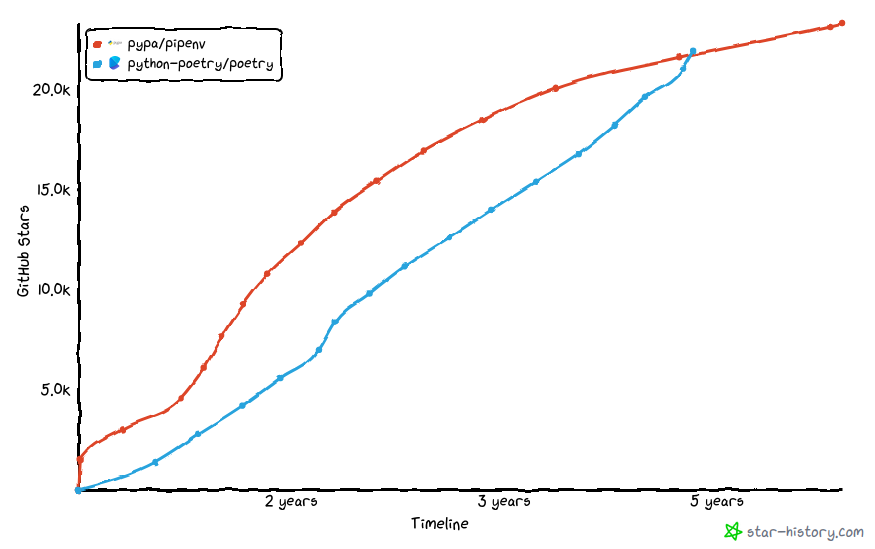
\includegraphics[width=\textwidth]{poetry-vs-pipenv}
                \end{tcolorbox}
                \caption{
                    Both a dependency managers comparison, and a good example
                    of trade-off: Pipenv is older, but Poetry has traction.
                }
            \end{figure}
        \end{column}
    \end{columns}
\end{frame}

\begin{frame}{Bots \& Hooks}
    \begin{columns}
        \begin{column}{0.05\textwidth}
        \end{column}
        \begin{column}{0.45\textwidth}
            Bots are useful as a category: checks that run automatically (and
            often asynchronously, events triggered) on the server.
            \vspace*{15pt}

            A useful example: scan dependencies and get updates about reported
            vulnerabilities.
            \vspace*{5pt}

            \vcinclude{dependabot}{width=50pt}
            \href{https://github.com/dependabot}{\textbf{Dependabot}}:
            Automated
            dependency updates.

            \href{https://probot.github.io/}{\textbf{Probot}}: an entire kit to
            build GitHub apps.
            \vcinclude{probot}{width=50pt}
            \vspace*{5pt}

            {\itshape\small
                I never used myself, but if you need something like Dependabot,
                you can use it to make your custom one (workflows can already
                do a lot).
            }
        \end{column}
        \begin{column}{0.45\textwidth}
            \begin{figure}
                \centering
                
\includegraphics[width=0.4\textwidth]{hooks}
            \end{figure}
            \href{https://git-scm.com/book/en/v2/Customizing-Git-Git-Hooks}{Git
            hooks} are another important help to \textbf{automate} and
            \textbf{ensure} routine \textbf{maintenance} (formatting, checks,
            \dots).\newline

            They are simple \textbf{executable scripts}\footnote{
                Not automatically installed at clone time, not to run unknown
                code.
            }, triggered by Git events (built-in feature, active as client and
            server).
            \vspace*{10pt}

            \href{https://pre-commit.com/}{\texttt{pre-commit}} is a framework
            to manage them.
            \vcinclude{pre-commit}{width=50pt}
            \vspace*{10pt}

            It is absolutely not required, but makes it much simpler to reuse
            hooks (especially community popular ones).
            Almost a \enquote{package manager for pre-commit hooks}.
            \vspace*{15pt}
        \end{column}
        \begin{column}{0.05\textwidth}
        \end{column}
    \end{columns}
\end{frame}

\begin{frame}[standout]
    Thanks for your attention!
\end{frame}

\appendix

\begin{frame}{Template}
    \begin{columns}
        \begin{column}{0.5\textwidth}
            
        \end{column}
        \begin{column}{0.5\textwidth}
            
        \end{column}
    \end{columns}
\end{frame}

\begin{frame}[fragile]{Poetry tutorial \& references}
    \begin{columns}
        \begin{column}{0.1\textwidth}
        \end{column}
        \begin{column}{0.4\textwidth}
            Tutorial
            \begin{lstlisting}[language=bash,style=mystyle]
# install dependencies
poetry install
# add dependency
poetry add mypackage
# add dependency to given group
poetry add mypackage -G mygroup

# generate lockfile
poetry lock
# update dependencies
poetry update

# run command in environment
poetry run mycommand
# enter shell inside environment
poetry shell\end{lstlisting}
        \end{column}
        \begin{column}{0.4\textwidth}
            References
            \lipsum[1]
        \end{column}
        \begin{column}{0.1\textwidth}
        \end{column}
    \end{columns}
\end{frame}


\begin{frame}{Store Knowledge}
    \begin{columns}
        \begin{column}{0.5\textwidth}
            Better than internal wiki $\to$ internal Q\&A.

            Use GitHub discussions for this.

            When a colleague give you an answer: consider to write it down in
            the discussions (for your future self, and the other colleagues).
            Even easier: make the question directly in a discussion.
        \end{column}
        \begin{column}{0.5\textwidth}
            When things consolidate:

            \begin{description}
                \item[\emoji{star} favorite] add to the docs (even developers docs)
                \item[internal] to keep internal add to a wiki repository
                  (still on GitHub -> maintain a unique platform).
            \end{description}

            In case: also Projects might be useful, to have a board for
            discussing status and priorities.
        \end{column}
    \end{columns}
\end{frame}


\end{document}
